\documentclass[12pt,oneside,letterpaper]{article}

\usepackage[canadien]{babel}
\usepackage[utf8]{inputenc}
\usepackage[T1]{fontenc}
\usepackage{lmodern}
\usepackage{graphicx}
\usepackage[letterpaper]{geometry}
\usepackage{caption}
\usepackage{amsmath}
\usepackage{subfig}
\usepackage{mhchem}
\usepackage{hyperref}
\usepackage[all]{hypcap}


\addto\captionsfrench{\def\tablename{Tableau}}
\captionsetup{font=small,labelfont=bf,margin=0.1\textwidth}
\pagestyle{myheadings}
\markboth{GPH-2006/PHY-2002~---~Fonctionnement~d'une~pile~électrochimique}{GPH-2006/PHY-2002~---~Fonctionnement~d'une~pile~électrochimique}


\begin{document}


\title{\textbf{Complément}\\Fonctionnement d'une pile électrochimique}
\author{Jean-Raphaël Carrier \& Claudine Allen}
\date{}
\maketitle


\section{Oxydoréduction}

L'oxydoréduction est une réaction chimique au cours de laquelle se produit un échange d'électrons. Comme son nom l'indique, elle est la combinaison de deux demi-réactions : l'oxydation et la réduction.

L'oxydoréduction apparaît en présence d'un réducteur (un donneur d'électrons) et d'un oxydant (un accepteur d'électrons). Il ne faut pas se mêler : le réducteur est l'élément qui se fait oxyder, alors que l'oxydant se fait réduire. Un élément peut autant être réducteur qu'oxydant, cela dépend du contexte : le meilleur accepteur d'électrons sera l'oxydant et l'autre sera le réducteur.

Le terme «réduction» vient du fait que l'oxydant voit son numéro d'oxydation diminuer (par exemple, l'oxygène neutre O devient un ion négatif O\up{2-}). Cette diminution de l'état d'oxydation est égale au nombre d'électrons que chaque oxydant aura capté. Les meilleurs réducteurs sont les éléments (ou les composés) qui «donnent» plus facilement leurs électrons : c'est le cas des métaux, plus particulièrement les alcalins.

Le terme «oxydation» vient du fait que cette demi-réaction est très souvent produite en présence d'oxygène, qui est un excellent oxydant. On n'a qu'à penser aux métaux qui rouillent (i.e. se font oxyder) en présence d'oxygène. Cependant, l'oxygène se fait réduire par ces métaux. Les meilleurs oxydants sont les éléments (ou les composés) qui «volent» plus efficacement les électrons des autres : c'est le cas des non-métaux, plus particulièrement les halogènes.

Voici deux exemples d'oxydoréduction:
\begin{center}
Oxydation: Cu = Cu\up{2+} + 2\,e\up{--}\\
Réduction: \ce{O2} + 4\,e\up{--} = 2\,O\up{2--}\\
Bilan: 2\,Cu + \ce{O2} $\rightarrow$ 2\,CuO
\end{center}

\begin{center}
Oxydation: Fe\up{2+} = Fe\up{3+} + e\up{--}\\
Réduction: Ce\up{4+} + e\up{--} = Ce\up{3+}\\
Bilan: Ce\up{4+} + Fe\up{2+} $\rightarrow$ Ce\up{3+} + Fe\up{3+}
\end{center}


\section{Pile électrochimique}

Lors d'une réaction d'oxydoréduction, les électrons vont du réducteur vers l'oxydant. Ce déplacement d'électrons peut donner naissance à un courant électrique.

Une pile électrique standard abrite une réaction d'oxydoréduction entre deux matériaux, dont l'un (le réducteur, qu'on appelle anode) peut facilement céder ses électrons et l'autre (l'oxydant, qu'on appelle cathode) les accepte volontiers. Chaque demi-réaction se produit dans une solution électrolytique où il y a échange d'électrons entre les électrodes, qui sont souvent métalliques, et les ions en solution. Un pont salin assure l'équilibre des charges entre les deux solutions ; les ions peuvent circuler dans le pont salin, mais pas le solvant. Lorsque la cathode et l'anode sont reliées au moyen d'un fil conducteur, il y a circulation d'un courant électrique continu.

\begin{figure}[h]
\begin{center}
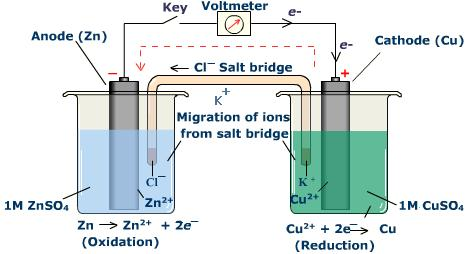
\includegraphics[width=0.65\textwidth]{ElectricCell}
\caption{\label{Pauling}Réaction d'oxydoréduction entre la cathode et l'anode d'une pile électrique. Un pont salin assure la neutralité du solvant, alors qu'un fil conducteur permet aux électrons de circuler de l'anode vers la cathode. Image provenant du site \texttt{http:\textbackslash\textbackslash www.tutorvista.com}.}
\end{center}
\end{figure}

La valeur du courant dépendra de la différence de potentiel entre la cathode et l'anode (bonne vieille loi d'Ohm : $v=R\,i$, où $R$ est la résistance du fil). Quant à elle, la différence de potentiel dépendra directement des matériaux utilisés pour l'anode et la cathode.


\section{Façons de comparer les électrodes}

Il existe plusieurs paramètres pour quantifier l'efficacité à générer une différence de potentiel de différentes combinaisons anode--cathode, mais tous se basent sur le même concept : c'est en combinant un bon donneur d'électrons à un bon accepteur d'électrons que la différence de potentiel sera la plus élevée. Trois concepts seront abordés dans ce document : le potentiel d'oxydoréduction, l'électronégativité et le travail de sortie.


\subsection{Potentiel d'oxydoréduction}

Le potentiel d'oxydoréduction, ou potentiel redox, est une façon de quantifier la réactivité des espèces chimiques entre elles. Noté $E$, c'est une grandeur empirique exprimée en volts et dont les mesures (potentiel standard) sont prises par rapport au couple proton/hydrogène (H\up{+}/\ce{H2}). Le tableau~\ref{tab-pot-redox} illustre quelques valeurs de potentiel standard.

\begin{table}[h]
\begin{center}
\begin{tabular}{|c|c|c|}
\hline
\textbf{Demi-équation} & \textbf{Potentiel standard~($\mathbf{E^0}$)} \\
\hline
Li\up{+} + e\up{--} = Li & $-3,\!0401$~V \\
\hline
Na\up{+} + e\up{--} = Na & $-2,\!71$~V \\
\hline
Al\up{3+} + 3\,e\up{--} = Al & $-1,\!66$~V \\
\hline
Fe\up{2+} + 2\,e\up{--} = Fe & $-0,\!44$~V \\
\hline
2\,H\up{+} + 2\,e\up{--} = \ce{H2} & $\equiv0$~V \\
\hline
Ag\up{+} + e\up{--} = Ag & 0,7996~V \\
\hline
Au\up{3+} + 3\,e\up{--} = Au & 1,52~V \\
\hline
Au\up{+} + e\up{--} = Au & 1,83~V \\
\hline
\ce{F2} + 2\,e\up{--} = 2\,F\up{--} & 2,87~V \\
\hline
\end{tabular}
\end{center}
\caption{\label{tab-pot-redox}Quelques exemples de potentiel standard. Ces valeurs sont obtenues à une température de 25~$^{\circ}$C, à une pression de 1~atm et avec une concentration effective de 1~mol/L pour chaque espèce aqueuse.}
\end{table}

Il est à noter que les potentiels les plus grands positivement sont associés aux meilleurs oxydants, et les plus grands négativement aux meilleurs réducteurs. On peut calculer le potentiel d'oxydoréduction d'une réaction complète en soustrayant le potentiel standard de la réduction à celui de l'oxydation:
\begin{equation}
E_{\mathrm{redox}}=E^0_{\mathrm{ox}}-E^0_{\mathrm{red}}.
\end{equation}
Par exemple, le potentiel d'oxydoréduction d'une pile dont les électrodes sont de l'aluminium (réducteur) et de l'argent (oxydant) est:
\begin{gather*}
E_{\mathrm{Ag/Al}}=E^0_{\mathrm{Ag}}-E^0_{\mathrm{Al}}\\
E_{\mathrm{Ag/Al}}=0,\!7996~\mathrm{V}+1,\!66~\mathrm{V}=2,\!46~\mathrm{V}.
\end{gather*}


\subsection{Électronégativité}

L'électronégativité d'un élément est sa capacité à capter des électrons afin de former des ions négatifs. Les éléments avec une forte électronégativité sont donc d'excellents oxydants et \textit{vice versa}. Ainsi, plus la différence d'électronégativité entre l'anode et la cathode est grande, plus la différence de potentiel aux bornes de la pile sera importante. La figure~\ref{Pauling} illustre l'électronégativité des différents atomes du tableau périodique selon l'échelle de Pauling, qui va de 0,7 (francium : meilleur réducteur) à 4 (fluor : meilleur oxydant).

\begin{figure}[h]
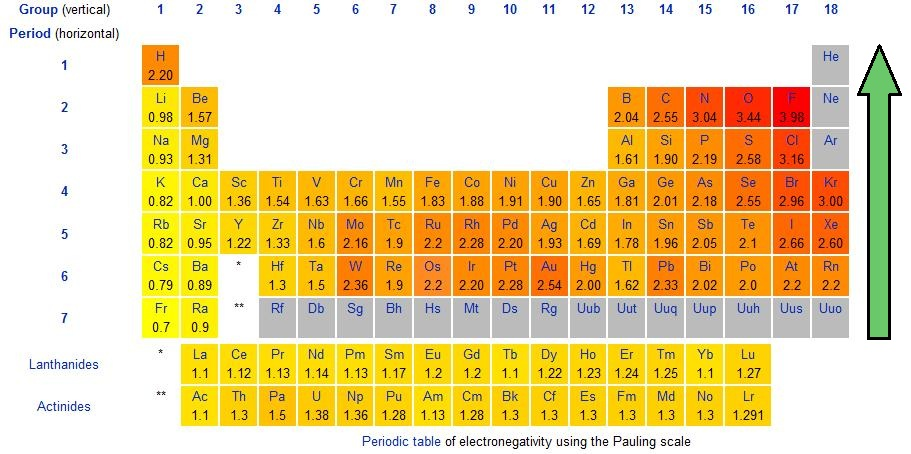
\includegraphics[width=\textwidth]{pauling-scale}
\caption{\label{Pauling}Tableau périodique de l'électronégativité. La flèche indique la tendance générale d'augmentation de l'électronégativité avec la diminution de la taille des atomes.}
\end{figure}


\subsection{Travail de sortie}

L'électronégativité est un paramètre qui touche presque tous les atomes du tableau périodique, mais de façon individuelle : ce paramètre quantifie les interactions entre des atomes isolés. Puisque les électrodes sont des solides métalliques et non des atomes isolés, la notion de \textit{travail de sortie} devient pertinente.

Il faut fournir de l'énergie pour arracher un électron à un métal. Ce travail doit être assez grand, d'une part, pour supplanter les forces d'attraction qui lient l'électron à l'atome et, d'autre part, pour compenser les pertes d'énergie cinétique causées par les collisions que subira l'électron sur son chemin vers la sortie hors du métal. Cependant, certains électrons sont liés plus solidement et certains perdront plus d'énergie cinétique que d'autres. Le travail de sortie (en anglais : \textit{work function}) est l'énergie minimale requise pour arracher un électron à la surface d'un métal. %%Un faible travail de sortie sera associé à un bon réducteur, alors qu'un grand travail de sortie sera associé à un bon oxydant. Ainsi, pour faire une pile efficace, il faut une différence entre les valeurs de travail de sortie aussi grande que possible.
Il existe une relation linéaire entre le travail de sortie et l'électronégativité. %La pente de cette relation linéaire est toutefois différente pour les métaux alcalins et alcalino-terreux et pour les métaux de transition.

La valeur du travail de sortie dépend du milieu dans lequel baigne le métal. L'énergie nécessaire pour prendre un électron d'un métal et l'apporter dans le vide n'est pas la même que l'énergie qui serait nécessaire pour apporter le même électron dans une solution électrolytique.


\end{document}
